Le module de mémoire se décompose en trois parties :
\begin{itemize}
\item la mémoire à court terme,
\item la mémoire épisodique,
\item la mémoire sémantique.
\end{itemize}

\subsection{Mémoire à court terme}

La mémoire à court terme est le module avec lequel communiquent les modules d'analyse et de raisonnement. Elle a un rôle de \emph{buffer} permettant de stocker temporairement les données soumises par le module d'analyse poussé, et sont fournis au module de raisonnement.

L'accès aux ressources stockées en mémoire sémantique ou épisodique se fait également par la mémoire à court terme ; elle peut être décrite comme l'interface mémoire.

\subsection{Mémoire épisodique}
\label{conception_memoire_episodique}

La mémoire épisodique stocke des parties et des coups. Tous les éléments sont datés au moment de l'ajout et peuvent être parcourus par ordre chronologique inversé (du plus récent au plus ancien).

Cette mémoire est structurée sous la forme d'une double liste chaînée :
\begin{itemize}
\item liste chaînée de parties, avec accès à la dernière partie jouée, chaque partie donnant accès à son dernier coup joué et la partie précédente,
\item liste chaînée de coups par partie, avec, pour chaque coup, accès au coup précédent.
\end{itemize}

\begin{figure}[H]
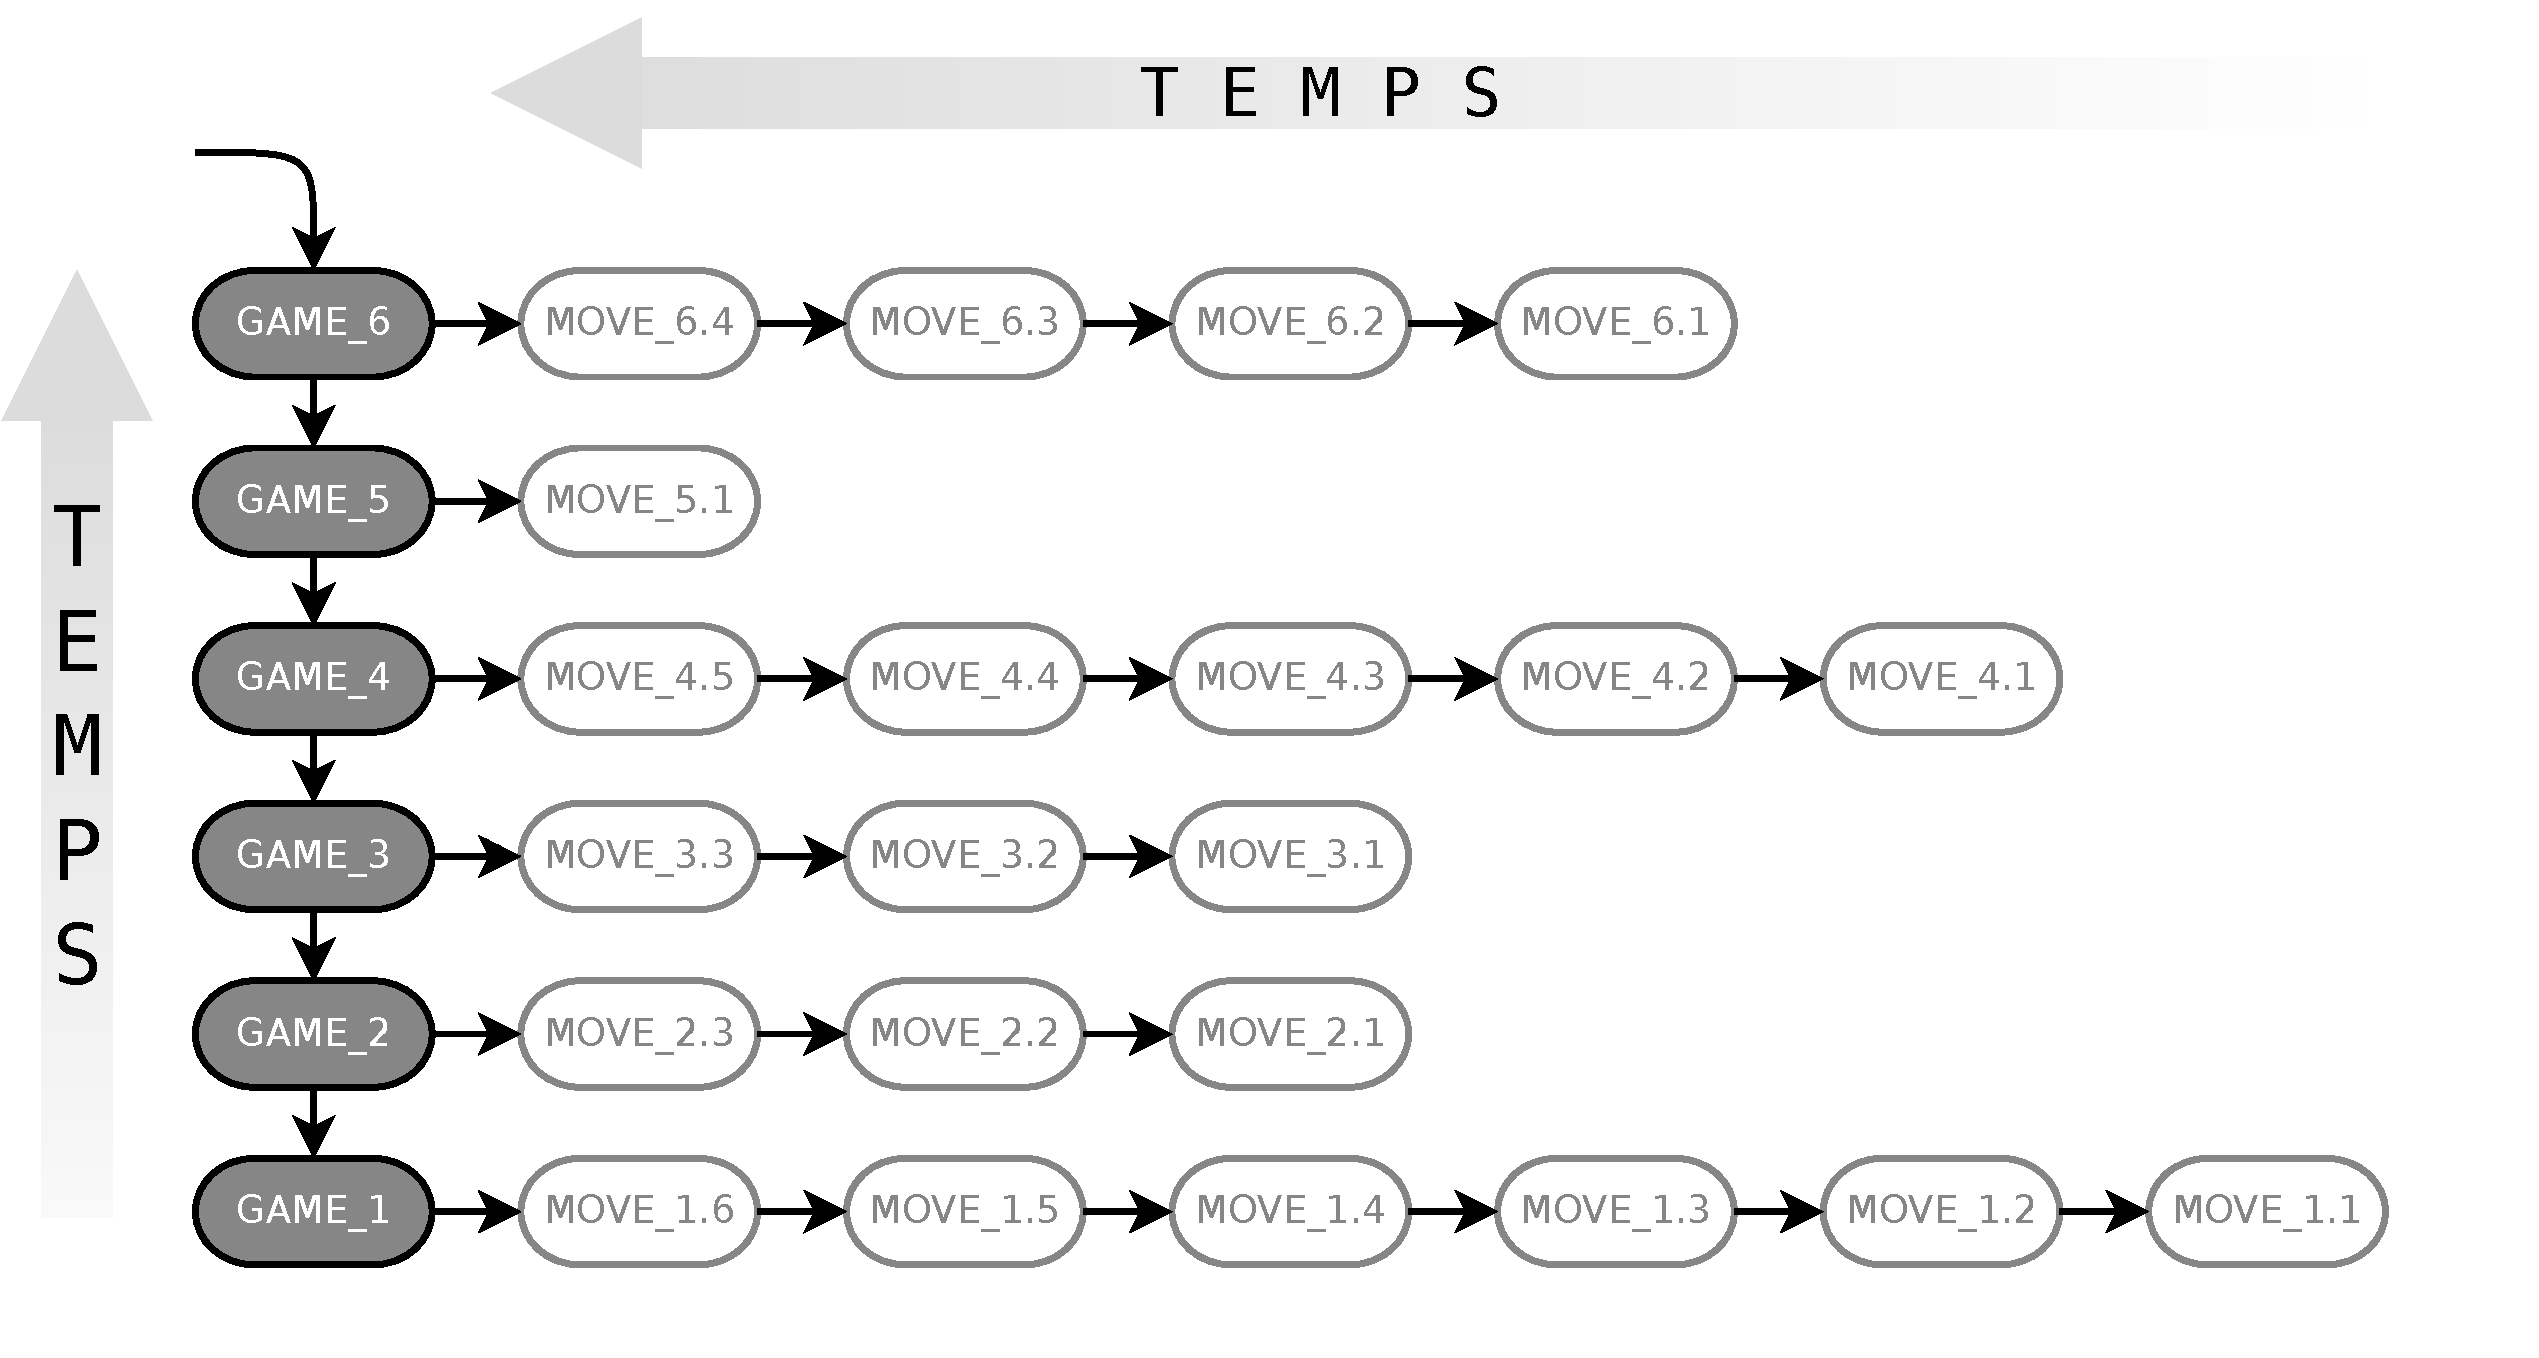
\includegraphics[width=\textwidth]{files/memoire/episodic_general}
\caption{Représentation de la mémoire, sous la forme d'une double liste chaînée avec accès par ordre chronologique inversé}
\end{figure}

\subsection{Mémoire sémantique}
\label{conception_memoire_semantique}

La mémoire sémantique permet le stockage :
\begin{itemize}
\item des plateaux rencontrés lors des parties,
\item des formes remarquables ajoutées au fil du temps par le module  d'introspection,
\item des relations entre les plateaux et les formes.
\end{itemize}

La structure d'une telle mémoire peu être vue comme :
\begin{itemize}
\item une matrice de booléens, chaque ligne correspondant à un plateau, et chaque colonne à une forme, $(x,y)=TRUE$ signifiant la présence de la forme y dans le plateau x,
\begin{figure}[H]
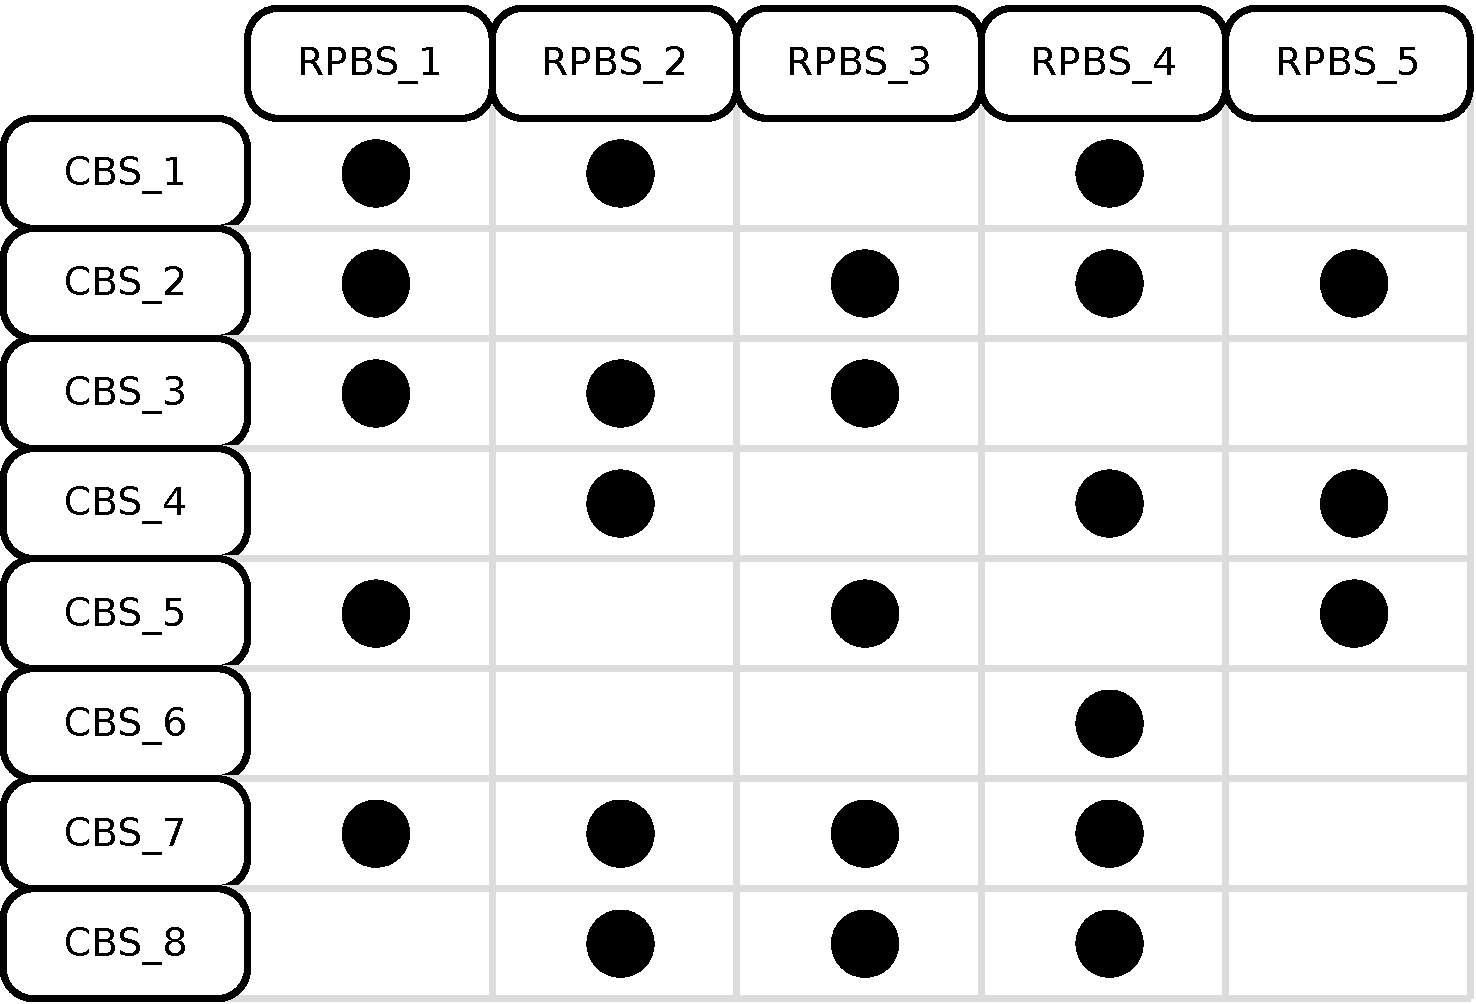
\includegraphics[width=\textwidth]{files/memoire/context_matrix}
\caption{Représentation de la mémoire sémantique sous forme matricielle.}
\end{figure}


\item un graphe biparti avec présence d'un arc x $\rightarrow$ y signifiant la présence de la forme y dans le plateau x.
\begin{figure}[H]
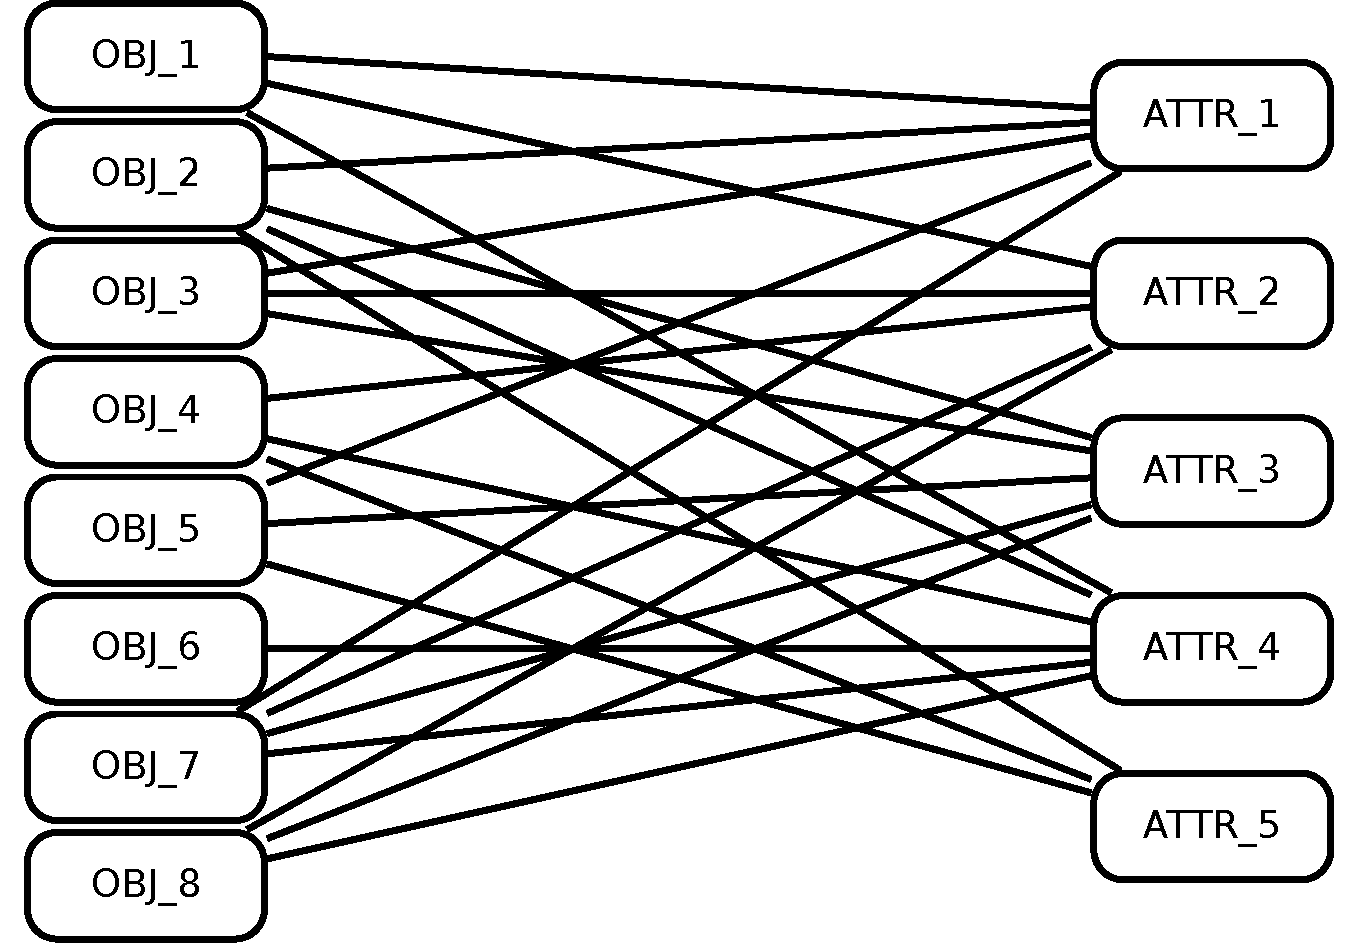
\includegraphics[width=\textwidth]{files/memoire/context_graph}
\caption{Représentation de la mémoire sémantique sous la forme d'un graphe biparti.}
\end{figure}
\end{itemize}